\documentclass[20pt,landscape]{foils}
\usepackage{amsmath, amssymb, amsthm}
\usepackage{color}
\usepackage{hyperref}
%\usepackage{pause}
\usepackage{graphicx}
\usepackage{epsfig}
%\usepackage{geometry}
%\geometry{headsep=3ex,hscale=0.9}
\newcommand{\bd}{\textbf}
\newcommand{\no}{\noindent}
\newcommand{\un}{\underline}
\newcommand{\bi}{\begin{itemize}}
\newcommand{\ei}{\end{itemize}}
\newcommand{\be}{\begin{enumerate}}
\newcommand{\ee}{\end{enumerate}}
\newcommand{\bc}{\begin{center}}
\newcommand{\ec}{\end{center}}
\newcommand \h {\hspace*{.3in}}
\newcommand{\bul}{\hspace*{.3in}{\textcolor{red}{$\bullet$ \ }}}
\newcommand{\xbar}{\bar{x}}
\rightheader{Stat 330 (Fall 2016): slide set 7}

\begin{document}
\LogoOff

\foilhead[1.3in]{}
\centerline{\LARGE \textcolor{blue}{Slide set 7}}
\vspace{0.3in}
\centerline{\large Stat 330 (Fall 2016)}
\vspace{0.2in}
\centerline{\tiny Last update: \today}
\setcounter{page}{0}

\foilhead[-.8in]{\textcolor{blue}{Random Variables}}
\no  {\textcolor{magenta}{Intuitive idea:}  {\textcolor{cyan}{If the value of a numerical variable depends on the outcome of an
experiment, we call the variable a {\it random variable}.}} \\[.1in]
{\textcolor{red}{Random Variable }}
A function $X: \Omega \mapsto \mathbb{R}$ is called a random variable.\\[.1in] 
%\no {\textcolor{magenta}{Standard notation:} Denote random variables by capital letters from the end of the alphabet.\\[.1in]   
\no   {\textcolor{magenta}{Example:  Very simple Dartboard}}\\[.01in]
\bc
\includegraphics*[scale=0.4]{dartboard.pdf}\\[.01in]
\ec
\no {\textcolor{cyan}{Imagine we throw three darts on this board one by one and we are interested in the number of times the
red area has been hit. This count is a random variable!}}\\[.1in]
\no Also note that $P(\text{red})=\frac{1}{9}$ on any throw.
\foilhead[-.8in]{\textcolor{blue}{Dartboard (continued...)}}
\no  More formally:\\[.1in] 
\no {\textcolor{cyan}{We define $X$ to be the function that assigns the number of times that the red area is hit in a sequence of three throws.}\\[.1in]
\no $X(\omega)=  k$, if the outcome $\omega$ has $k$ hits to the red area, and $3-k$ hits to the gray area.\\[.1in]
\no $X(\omega)$ is then an integer between 0 and 3 for every possible  sequence of throws of 3 darts.\\[.1in]
\no That is, the set of possible values for $X(\omega)$ is $\{0,1,2,3\}$\\[.1in]   
 \no  {\textcolor{magenta}{Notation:} To avoid cumbersome notation, we write
$$\{X = x\}$$ 
for the event
\[
\{ \omega | \omega \in \Omega\ \text{ and }\ X(\omega) = x \}.
\]
    
   
\foilhead[-.8in]{\textcolor{blue}{Practice with notation}}   
\no   {\textcolor{magenta}{Example}} {\textcolor{cyan}{Suppose, 8 bits are sent through a communication channel.
Each bit has a certain probability to be received incorrectly. We are interested in the number of bits that are received incorrectly.}}\\[.1in]
\no Use random variable $X$ to ``count'' the number of wrong bits received.
 $X$ assigns a value between 0 and 8 to each sequence in the sample space.\\[.1in]
\no That is, the possible values for $X$  are $\{0,1,2,3,4,5,6,7,8\}$\\[.1in]
\no Examples of events and equivalent expressions using $X$. \\[.1in]
\bul No wrong bits received: $\{X=0\}$\\[.1in]
\bul At least one wrong bit received: $\{X\geq 1\}$\\[.1in]
\bul Exactly 2 wrong bits received: $\{X=2\}$\\[.1in]
\bul Between 2 and 7 wrong bits (inclusive) received: $\{2\leq X\leq 7\}$   
     
\foilhead[-.8in]{\textcolor{blue}{Image of R.V.: all possible values $X$ can take}}
\no {\textcolor{magenta}{Definition:}} The image of a random variable $X$ is defined as
\no \hspace*{1in} $Im(X) := \{x: x=X(\omega) \text{ for some }\omega \in \Omega \}.$ \\[.1in]
%\no {\textcolor{red}{Depending on whether or not the image of a random variable is
%countable, we distinguish between {\it discrete} and {\it continuous}
%random variables. }}
   \begin{enumerate}
	\item Put a disk drive into service, measure $Y$ = ``time till
	the first major failure''.\\[.1in]
		$Im(Y) = (0, \infty)$.\\[.1in]
    image of $Y$ is an interval (uncountable image) $\rightarrow Y$ is a
  continuous random variable.
	\item Communication channel: $X$ = ``\# of incorrectly received bits''\\[.1in]
		$Im(X) = \{ 0,1,2,3,4,5,6,7,8 \}$ is a finite set $\rightarrow X$ is
	a discrete random variable.
    \end{enumerate}
    
    
    
\foilhead[-.8in]{\textcolor{blue}{Discrete R.V.s}}
\no \bul Assume $X$ is a discrete random variable. The image of $X$ is
therefore countable and can be written as $\{ x_{1}, x_{2}, x_{3},
\ldots \}$\\[.1in]
\no \bul Very often we are interested in probabilities of the form $P(X=x)$.
\no We can think of this expression as a function, that yields different
probabilities depending on the value of $x$.\\[.1in]
\no {\textcolor{magenta}{Example: Dartboard}}  {\textcolor{cyan}{ What is the probability that you hit the red square exactly twice in 3 throws?}}\\[.1in]
\no The event ``exactly 2 reds'' is formally written as $\{\omega : X(\omega)=2$\}, and with the
simpler notation for this event  is $X=2$.\\[.1in]
\no $P(\text{2 reds}) = P(X=2)$ \\[.1in]
\no \hspace*{1.2 in} $ = P(RRG \text{ or } RGR \text{ or } GRR)$ \\[.1in]
\no \hspace*{1.2 in} $ = P(RRG)+P(RGR)+P(GRR)$\\[.1in] 
\no \hspace*{1.2 in} $ = \frac{1}{9}\cdot\frac{1}{9}\cdot\frac{8}{9}+\frac{1}{9}\cdot\frac{8}{9}\cdot\frac{1}{9}+\frac{8}{9}\cdot\frac{1}{9}\cdot\frac{1}{9}=?$



\foilhead[-.8in]{\textcolor{blue}{Probability Mass Function}}
\no \no  {\textcolor{cyan}{Definition: Probability Mass Function, PMF} \\[.1in]
\no {\textcolor{red}{   The function $p_{X}(x) := P(X=x)$ is called the {\it probability mass function
    of $X$}. }}
 
 
   \no \no  {\textcolor{cyan}{Properties of PMF:} \\[.1in]
 $p_{X}$ is the pmf of $X$, if and only if
    \begin{itemize}
	\item[(i)] $0 \le p_{X}(x) \le 1$ for all $x \in \{ x_{1}, x_{2}, x_{3},
\ldots \}$ ({all values must be between 0 and 1})
        \item[(ii)]  
        $\sum_{i}p_{X}(x_{i}) = 1$ ({the sum of all values is 1})
    \end{itemize}
    
    
  \foilhead[-.8in]{\textcolor{blue}{Examples:}} 
   \no {\textcolor{red}{These properties give us an easy method to check, whether a function is a
probability mass function }}  \\[.1in]
   \no {\textcolor{magenta}{Experiment:}    Which of the following functions is a valid probability mass
    function?
    \begin{enumerate}
    \item
    	\begin{tabular}{c|ccccc}
		$x$ & -3 & -1 & 0 & 5 & 7  \\
		\hline
		$p_{X}(x)$ & 0.1 & 0.45 & 0.15 & 0.25 & 0.05  \\
	\end{tabular}
    \item
    	\begin{tabular}{c|ccccc}
		$y$ & -1 & 0 & 1.5 & 3 & 4.5 \\
		\hline
		$p_{Y}(y)$ & 0.1 & 0.45 & 0.25 & -0.05 & 0.25  \\
	\end{tabular}
    \item
    	\begin{tabular}{c|ccccc}
		$z$ & 0 & 1 & 3 & 5 & 7  \\
		\hline
		$p_{Z}(z)$ & 0.22 & 0.18 & 0.24 & 0.17 & 0.18  \\
	\end{tabular}
    \end{enumerate}
    
    
 \foilhead[-.8in]{\textcolor{blue}{More Examples of Discrete R.V.'s}}
 \no {\textcolor{magenta}{Example: }} {\textcolor{cyan}{Roll of a fair die}}\\[.1in] 
\no 	Let $Y$ be the number of spots on the upturned face of a die.\\[.15in]  	
\no Obviously, $Y$ is a random variable with image $Im(Y)=\{1,2,3,4,5,6\}$.	\\[.1in] 
\no Assuming, that the die is a fair die means, that the outcomes of 
each face turning up are equally likely i.e.,
	probabilities of each face turning up are equal.\\[.1in]  
\no The probability mass function for $Y$ therefore is \\[.1in] 
\hspace*{1in}\begin{tabular}{c|cccccc}
		$x$ & 1 & 2 & 3 & 4 & 5& 6 \\
		\hline 
		$p_{X}(x)$ & $\frac{1}{6}$  & $\frac{1}{6}$ & $\frac{1}{6}$ & $\frac{1}{6}$ & $\frac{1}{6}$ & $ \frac{1}{6} $ 
\end{tabular}

%\no Checkout pmf's in  Examples 3.1 and 3.3 from Baron's book.
   
 \foilhead[-.8in]{\textcolor{blue}{More Examples of Discrete R.V.'s}}
 \no {\textcolor{magenta}{Example: }} {\textcolor{cyan}{Roll of a doctored die}}\\[.1in] 
 \begin{minipage}[t]{6in} 
	    The diagram shows all six faces of a particular die.
	    If $Z$ denotes the number of spots on the upturned face after 
	    toss this die,
	    what is the probability mass function for $Z$?
	    
	    {\it Assuming, that each face of the die appears with the same 
	    probability, we have 1 possibility to get a 1 or a 4, and two 
	    possibilities for a 2 or 3 to appear, which gives a probability 
	    mass function for $Z$ as:
	     \[
	    \begin{array}{l||c|c|c|c}
		z & 1 & 2 & 3 & 4 \\ \hline
		p(z) & 1/6 & 1/3 & 1/3 & 1/6 
	    \end{array}
	    \]
	    }
	\end{minipage}
	\hfill
	\begin{minipage}[t]{2in}
	    	\vspace{0in}
            	 \centerline {
            	 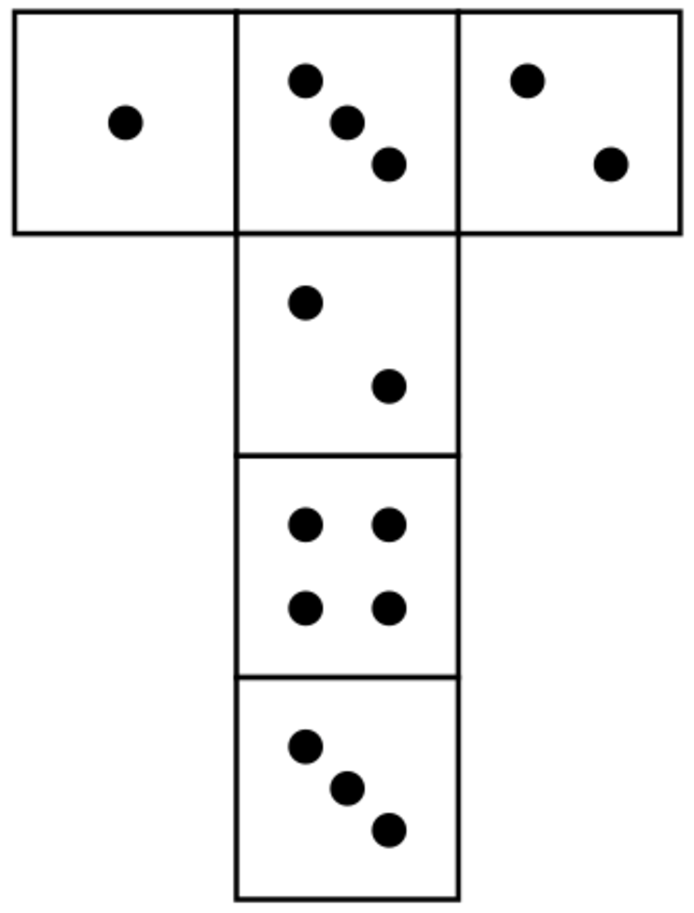
\includegraphics[width=2in]{die-faces.pdf}
		}
	\end{minipage}
 


\foilhead[-.8in]{\textcolor{red}{Statistics of R.V.s}}
\no {\textcolor{magenta}{Gamblers Luck!:}}
{\textcolor{cyan}{Toss a die. Let $X$ be the number of spots turned up, then if}}\\[-.2in]
\[
X = \left\{ \begin{array}{rll}
& 1,\ 3\ \text{or}\ 5 & \text{I pay you}\ \$ X\\
& 2\ \text{or}\ 4 & \text{you pay me}\ \$ 2X \\
& 6 & \text{no money changes hands.}
\end{array}
\right .
\]

\no {\textcolor{cyan}{What amount of money do I \emph{expect} to win?}}\\[.1in]
\no For that, we look at another function, $h(x)$, that counts the money I win with
respect to the number of spots:
\[
h(x) = \left\{ \begin{array}{rl}
-x & \text{ for } x = 1,3,5 \\
2x & \text{ for } x = 2,4 \\
0 & \text{ for } x = 6.
\end{array}
\right .
\]

   \foilhead[-.8in]{\textcolor{red}{Gambling Example Continued...}}\vspace*{.05in}
\begin{tabular}{@{In 1/6 of all tosses $X$ will be }c@{, and I will
gain }r@{ dollars}}
1 & -1\\[.05in]
2 & 4 \\[.05in]
3 & -3 \\[.05in]
4 & 8 \\[.05in]
5 & -5 \\[.05in]
6 & 0 
\end{tabular}

\no In total I expect to get\\[.15in] 
\hspace*{1in} $\frac{1}{6} \cdot (-1) + \frac{1}{6} \cdot
4 + \frac{1}{6} \cdot (-3) + \frac{1}{6} \cdot 8 + \frac{1}{6} \cdot
(-5) + \frac{1}{6} \cdot 0 = \frac{3}{6} = 0.5$\\[.15in]
\no dollars per play.\\[.1in]
\no In this example, we are calculating the \emph{expected value} of the function $h(X)$\\[.1in]
\no We denote this by $E(h(X))$ and define this mathematically in the next lecture.


\end{document}




